\documentclass{../exhibit}


%% Debi Stout and
%% Bart Snapp


\title{Pirate Codes}

%% Font
\usepackage{imfellEnglish}
\usepackage[T1]{fontenc}
\raggedright

\usepackage{background}

\backgroundsetup{
scale=1,
color=black,
opacity=0.4,
angle=0,
contents={%
  \includegraphics[height=\paperheight]{mapBackground.jpg}%%https://upload.wikimedia.org/wikipedia/commons/8/81/Nautical_chart_of_the_West_Indies_1797.jpg
  }%
}




%% For the context
%% https://tex.stackexchange.com/questions/86150/torn-page-effect/86151#86151
\usepackage{tikz}
\usetikzlibrary{decorations.pathmorphing}
\definecolor{paper}{RGB}{239,227,157}





\renewcommand{\maketitle}{ %
  \begin{center}
    \scalebox{8}{\thetitle}
  \end{center}
  
\begin{tabular*}{\textwidth}{c @{\extracolsep{\fill}} c}  
\resizebox{4in}{!}{\begin{minipage}[b]{3in}\huge\directions\end{minipage}} &
  \resizebox{4in}{!}{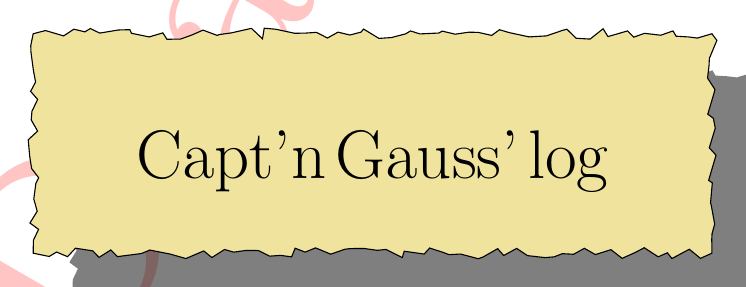
\begin{tikzpicture}[pencildraw/.style={ %
    decorate,
    decoration={random steps,segment length=4pt,amplitude=2pt}
    } %
]
\node[
preaction={fill=black,opacity=.5,transform canvas={xshift=.5cm,yshift=-.5cm}},
pencildraw,draw,fill=paper,text width=3in,inner sep=.5cm] 
{\begin{center}\Huge Capt'n Gauss' log \end{center}\vspace{.7cm} {\huge\context}};
\end{tikzpicture}}

\end{tabular*}

\vfill

\includegraphics[width=3in]{logoPirate.png}\hfill \includegraphics[width=2in]{bammLogo.png}


}


\begin{document}

\begin{context}

  Pirates be keepers of\\
  \hspace{1in}SECRETS \\
  With codes, we make do\\[1cm]

  Learn this code, and keep secrets\\
  \hspace{2in}too!
  
\end{context}

\begin{directions}\Large
  To Encode:
  \begin{itemize}
    \item Write a message. Convert it to numbers, using the wheel below.
    \item For each number in your message, draw a card,
      \begin{itemize}
      \item If the card is black, add its value
        to the number,
      \item If the card is red, subtract its value from the number,
      \end{itemize}
    \item Place the card at the bottom of the deck.
    \item Convert the number back to a letter, and move to the next number.
  \end{itemize}
      To Decode:
  \begin{itemize}
    \item Convert the message to numbers, using the wheel below.
    \item For each number in your message, draw a card,
      \begin{itemize}
      \item If the card is black, subtract its value
        to the number,
      \item If the card is red, add its value from the number,
      \end{itemize}
      \item Place the card at the bottom of the deck.
      \item Convert the number back to a letter, and move to the next number.
  \end{itemize}
\end{directions}

  \begin{example}
    \begin{center}
 \scalebox{.7}{\begin{tikzpicture}[x=1em,y=1em]
%   set up
    \pgfmathsetmacro\angdiv{360/26}
    \pgfmathtruncatemacro\caeser{0} % Input Caeser shift here! (positive for clockwise)
    \coordinate (n-0) at (90+\angdiv/2:7) {};
    \coordinate (m-0) at (90-\caeser*\angdiv+\angdiv/2:5) {};
%   draw Caeser diagram 
    \draw circle [radius=8] circle [radius=6.5] circle [radius=6]  circle [radius=4.5]
        \foreach \i in {0,...,25}{%
            ($({90-(\i-1/2)*\angdiv}:8)$) -- ($(({90-(\i-1/2)*\angdiv}:6.5)$)
            ($({90-(\i-1/2)*\angdiv}:4.5)$) -- ($(({90-(\i-1/2)*\angdiv}:6)$)
        };
    \foreach [count=\a from 0] \text in {A,B,...,Z}{
        \pgfmathtruncatemacro\b{\a+1}%
        \path [curved text=\text] (n-\a) arc [start angle=90-(\a-1/2)*\angdiv, delta angle=-\angdiv, radius=7] node (n-\b) {};
        %\path [curved text=\text] (m-\a) arc [start angle=90-(\a+\caeser-1/2)*\angdiv, delta angle=-\angdiv, radius=5] node (m-\b) {}; % Inner circle
    }
    \foreach [count=\a from 0] \text in {1,2,...,26}{
        \pgfmathtruncatemacro\b{\a+1}%
        %\path [curved text=\text] (n-\a) arc [start angle=90-(\a-1/2)*\angdiv, delta angle=-\angdiv, radius=7] node (n-\b) {};
        \path [curved text=\text] (m-\a) arc [start angle=90-(\a+\caeser-1/2)*\angdiv, delta angle=-\angdiv, radius=5] node (m-\b) {}; % Inner circle
    }
    \end{tikzpicture}}
\end{center}
\end{example}

\begin{mathConnections}
  https://bartsnapp.github.io/Math-Outreach-Exhibits/cypher/
\end{mathConnections}
\end{document}
